\documentclass[12pt]{article}

\usepackage{fullpage}
\usepackage{graphics}
\usepackage{tikz}
\usepackage[parfill]{parskip}
\usepackage[utf8]{inputenc}
\usepackage{etoolbox}

\newbool{alt}
\booltrue{alt}
%\boolfalse{alt}

% Standard things to include for math
\usepackage{amsmath,amssymb,amsfonts,amsthm}

\usepackage{wasysym}

\usepackage{enumitem}



\usepackage{geometry}
 \geometry{
 a4paper,
 top=2cm,
 bottom=2cm,
 left=2cm,
 right=2cm,
 }




% Some of Ebrahim's definitions
\newcommand{\done}{\\\hspace*{0pt}\hfill$\blacksquare$}
\def\N{\mathbb{N}}
\def\R{\mathbb{R}}
\def\Q{\mathbb{Q}}
\def\Z{\mathbb{Z}}
\def\e{\epsilon}
\newcommand{\seq}[1]{\left(#1\right)_{n\in\N}}
\newcommand{\Euc}[1]{\mathbb{R}^{#1}}
\newcommand{\pathvarNaked}{p}
\newcommand{\pathvar}{\vec{\pathvarNaked}}
\newcommand{\pathvarAlt}{\vec{q}}
\newcommand{\exercisesList}[2]{\textcolor{ForestGreen}{Exercises from WeBWorK HW#1: #2.}}
\newcommand{\exerciseText}[1]{\textcolor{ForestGreen}{Exercise: #1}}
\def\vx{\vec{x}}
\def\vu{\vec{u}}
\def\vv{\vec{v}}
\def\vw{\vec{w}}
\newcommand{\der}[2]{\frac{\textrm{d}#1}{\textrm{d}#2}}
\newcommand{\derOp}[1]{\der{\phantom{#1}}{#1}}
\newcommand{\pder}[2]{\frac{\partial #1}{\partial #2}}
\newcommand{\pderOp}[1]{\pder{\phantom{#1}}{#1}}
\newcommand{\colvectwo}[2]{\left[\begin{array}{c}#1\\#2\end{array}\right]}
\newcommand{\colvectwoXYVEC}[2]{\left[#1\right]\,\cbv{x} + \left[#2\right]\,\cbv{y}}
\newcommand{\colvecthree}[3]{\left[\begin{array}{c}#1\\#2\\#3\end{array}\right]}
\newcommand{\colvecfour}[4]{\left[\begin{array}{c}#1\\#2\\#3\\#4\end{array}\right]}
\newcommand{\colvecfourL}[4]{\left[\begin{array}{l}#1\\#2\\#3\\#4\end{array}\right]}
\newcommand{\norm}[1]{\left|\hspace{-1.5pt}\left|#1\right|\hspace{-1.5pt}\right|}
\def\grad{\vec{\nabla}}
\newcommand{\Dir}[3]{\operatorname{Dir}(#1,#2,#3)}
\newcommand{\D}[1]{\textrm{D}#1}
\def\vn{\vec{n}}
\newcommand{\cbv}[1]{\partial_{#1}}
\newcommand{\arrayBrackets}[2]{\left[ \begin{array}{#1} #2 \end{array} \right] }

\makeatletter
\newcommand*\dotp{\mathpalette\bigcdot@{.5}}
\newcommand*\bigcdot@[2]{\mathbin{\vcenter{\hbox{\scalebox{#2}{$\m@th#1\bullet$}}}}}
\makeatother



\newcommand{\ansbox}[2]{\raisebox{-.5\height}{\framebox(#1,#2){}}}

\def\endans{\hspace{1em}\ansbox{40}{40}}


\newcommand{\NEcheckbox}{ % Put check box on northeast corner of page
\begin{tikzpicture}[remember picture,overlay]
\path (current page.north east) ++(-1,-1) node[below left] {
{\small graded?} {\Large\Square}
};
\end{tikzpicture}
}

\newcommand{\LEFTcheckbox}{ % Put check box in the left margin
\\\begin{tikzpicture}[remember picture,overlay]
\path ++(-2,0) node[below left] {
 {\Large\Square}
};
\end{tikzpicture}
}

\newcommand{\LEFTcheckboxOwnLine}{ % Put check box in the left margin, use this one if on own line
\begin{tikzpicture}[remember picture,overlay]
\path ++(-2,0) node[below left] {
 {\Large\Square}
};
\end{tikzpicture}
}






\pagenumbering{gobble}
\begin{document}




% --- Score table ---

%\def\gap{\hspace*{2.5em}}
%
%\begin{tikzpicture}[overlay, remember picture]
%\path (current page.north east) ++(-1,-1) node[below left] {
%\begin{tabular}{c|c|c|c|c|c|c|c}
% 1 &  2 & 3 & 4 & 5 & 6 & 7 & $\Sigma$\\ \hline
% \gap & \gap & \gap & \gap & \gap & \gap & \gap & \gap \\
% \gap & \gap & \gap & \gap & \gap & \gap & \gap & \gap
%\end{tabular}
%};
%\end{tikzpicture}

% ---


\def\namepos{(current page.north west) ++(5,-0.8)}
\begin{tikzpicture}[overlay, remember picture]
\draw [black] \namepos rectangle ++(10,-1);
\draw [black] \namepos ++(0,-1.2) rectangle ++(10,-1);
%\draw [black] \namepos ++(0,-1.2) ++(0,-1.2) rectangle ++(10,-1);
%\draw [black] \namepos ++(0,-1.2) ++(0,-1.2) ++(0,-1.2) rectangle ++(10,-1);
\path \namepos ++(0,-0.4) node [left] {\textbf{Name:}};
\path \namepos ++(0,-0.4) ++ (0,-1.2) node [left] {\textbf{Perm:}};
%\path \namepos ++(0,-0.4) ++ (0,-1.2) ++ (0,-1.2) node [left] {\textbf{Seat Number:}};
%\path \namepos ++(0,-0.4) ++ (0,-1.2) ++ (0,-1.2) ++ (0,-1.2) node [left] {\textbf{ID Checker Name:}};
\end{tikzpicture}

\def\versionRowText{
\textit{version \ifbool{alt}{1}{2},row}
\raisebox{-3pt}{\framebox(15,15){A}}
}
\begin{tikzpicture}[overlay, remember picture]
\path (current page.north east) ++ (-2,-1.5) node [left]{}; %{\versionRowText};
\end{tikzpicture}



\vspace{5em}

\begin{center}\textbf{Math 34A Midterm 3, Summer 2022}

({\it 100 pts total})
\end{center}
\begin{enumerate}


%\newpage
%%%%%%%%%%% (1)
\newpage
\item Use the log table provided with this exam to answer the following questions:

\begin{enumerate}

\item ({\it 4 pts}) Find $\log(10) + \log(0.316)$.
\vfill

\hfill$ \ $ \ansbox{200}{70}

\item ({\it 4 pts}) If $\log(y)=6.3$, then find $y$. 
\vfill

\hfill$ y=\ $ \ansbox{200}{70}

\item ({\it 4 pts}) Find the average rate of change of $10^x$ between $x=0.7$ and $x=0.9$.
\vfill

\hfill$\frac{\Delta y}{\Delta x}= \ $ \ansbox{200}{70}
\end{enumerate}


\pagebreak
%%%%%%%%%%% (2)
\item Compute the following derivatives.
\begin{enumerate}
\item ({\it 4 pts}) $\displaystyle\frac{d}{dx}\left( 3x^5 - 2x^2 - 14\sqrt{x} \right)=$ \ansbox{200}{70} 
\vfill

\item ({\it 4 pts}) $\displaystyle\frac{d}{dx}\left( 4x^2 + 5e^{2x} - 5e^{3x} \right)=$ \ansbox{200}{70} 
\vfill

\item ({\it 4 pts}) Consider the function $$f(x) = \frac{a}{\sqrt[3]{x}} - \frac{b}{(e^{x})^2}$$ where $a$ and $b$ are constants. Find $f'(1)$. 
\vfill
\vfill

\hfill $ \ f'(1)= \ $ \ansbox{300}{70}
\end{enumerate}


%%%%%%%%%%% (3)
\newpage
\item This question is about the graph of the function
$$f(x)=2x^3 +3x^2 - 12x + 172.$$
\begin{enumerate}
\item ({\it 5 pts}) What is the slope of the graph at $x=0$?
\vfill

\hfill slope$ \ = \ $ \ansbox{200}{70}
\item ({\it 5 pts}) What is the equation of the tangent line to the graph at $x=2$? Use the form $y=mx+b$.
\vfill

\hfill$ \ y= \ $ \ansbox{200}{70}
\item ({\it 5 pts}) For which $x$ value(s) does the graph have 0 slope?
\vfill

\hfill$ \ x= \ $ \ansbox{200}{70}
\item ({\it 5 pts}) For which $x$ values is the graph $y=f(x)$ concave down? 
\vfill

\hfill \ansbox{200}{70}
\end{enumerate}

\newpage
%%%%%%%%%%% (4)
\item A large Nerf ball is launched upward from the top of a cliff. Its height (in meters) $t$ seconds after launch is modeled by the equation $$h(t)=-5t^2 + 30t + 50.$$ (In this problem we are ignoring horizontal movement.)
\begin{enumerate}
\item ({\it 7 pts}) Find the function which gives the velocity of the ball after $t$ seconds. 
\vfill

\hfill $ \ \ $ \ansbox{200}{70} 
\item ({\it 7 pts}) What is the initial height of the ball?
\vfill

\hfill $h \ = \ $ \ansbox{200}{70} \phantom{in} m
\item ({\it 7 pts}) What is the acceleration of the ball after 5 seconds?
\vfill

\hfill acceleration$ \ = \ $ \ansbox{200}{70} \phantom{in}m/s$^2$
\item ({\it 7 pts}) When does the ball stop rising and begin to fall? (Hint: What would the ball's speed be at that moment?)
\vfill

\hfill at$ \ t \ = \ $ \ansbox{200}{70} \phantom{in}s
\item ({\it 7 pts}) What was the ball's maximum height?
\vfill

\hfill $ \ h \ = \ $ \ansbox{200}{70} \phantom{in}m
\end{enumerate}



%%%%%%%%%%% (5)
\newpage
\item A bacteria colony on a petri dish is growing in the shape of a circle. After $t$ days, the radius of the circle is $t^2+2t$ mm.
\begin{enumerate}
\item ({\it 6 pts}) What is the area of the circle after $t$ days? \vfill

\hfill $A(t)=$\ \ansbox{200}{50} \phantom{i} mm$^2$\phantom{/day}
\bigskip
\item ({\it 7 pts}) How quickly is the area of the circle growing after $t$ days? \vfill

\hfill $A'(t)=$\ \ansbox{200}{50} \phantom{i} mm$^2$/day
\bigskip
\item ({\it 8 pts}) As time goes by will the area of the circle grow faster, slower, or does the area grow at a constant rate? Why? (Use calculus to justify your answer). 

\ansbox{.9\textwidth}{250} 

\end{enumerate}
\bigskip



%
%%%%%%%%%%%% (6)
%\item ({\it 6pts})  You have 600m of fencing for a rectangular field, but the field needs to also be 
%
%\parbox{.5\textwidth}{\vspace*{-30 pt} subdivided into 3 equal areas by fencing as shown in the figure to the right. If $\ell$ and $w$ (length and width) are the dimensions of your pen, the total combined fencing must be 600m, so
%    $$4\ell + 2w = 600.$$}
%    \parbox{.5\textwidth}{%
%      \vspace*{-10 pt}      
%      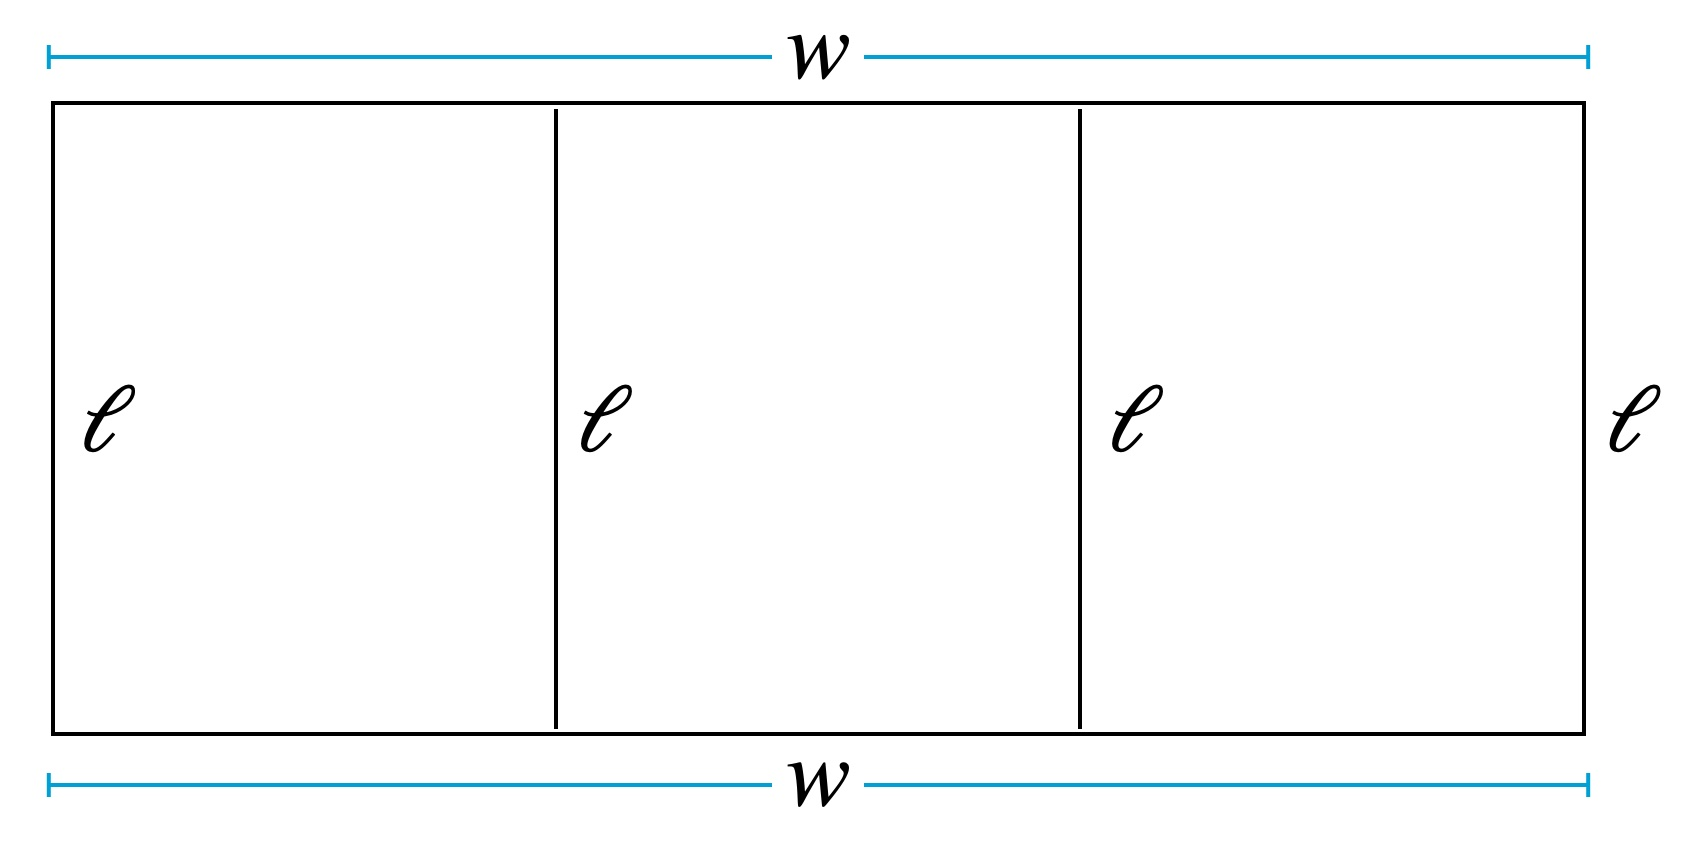
\includegraphics[width=.5\textwidth]{problem_6_figure}
%    }
%    
%    %Here there are two extra ``lengths'' to serve as dividers between the three subdivisions. \\
%    \begin{enumerate}
%    \item %You know the area of the pen in terms of $\ell$ and $w$. 
%    Express the \textbf{area} of the pen in terms of \underline{$\ell$ only}. \vfill
%
%    \hfill$A(\ell) =$\ \ansbox{190}{50} \phantom{i} m$^2$
%    \item Find the length that results in the largest area $A(\ell)$ for your field. \vfill
%
%    \hfill$\ell =$\ \ansbox{190}{50} \phantom{i} m\phantom{$^2$}
%    \item Use your answer in part (b) to find the maximum area for your field. \vfill
%
%    \hfill $A_{\text{max}} =$\ \ansbox{190}{50} \phantom{i} m$^2$
%    \end{enumerate}
%
%    \newpage
%
%












\end{enumerate}



\end{document}
